En esta sección, mostraremos el primer experimento realizado. Este consistió en aplicar un modelo de regresión lineal de cada variable social sobre el \entrainment, sin desagregar los datos por sesión y hablante.

Una variación que usamos en el presente experimento (y en el posterior) es utilizar como variable dependiente el valor absoluto del \entrainment, en base a estudios que sugieren que los interlocutores pueden también diferenciarse como un rasgo positivo en la conversación.

\section{Nuestro modelo de regresión}

Dada una variable acústica/prosódica (por ejemplo, el pitch o la intensidad), queremos investigar la relación entre entrainment y las distintas variables sociales medidas. Sea $V$ una variable social de las enumeradas en la tabla \ref{sec:panel_data}. Sean $E_1, \ldots, E_n$ los valores de entrainment para el set de datos que definimos en la sección \ref{sec:panel_data}, y sean $V_1, V_2, \ldots V_n$ los valores de la variable social de cada conversación.

Sobre éstas variables es que planteamos nuestro modelo de regresión lineal clásica, para analizar qué relación hay tomando como variable ``fija'' al \entrainment, y como variable dependiente a la variable social. El problema, entonces, es hallar estimadores $\widehat{\beta_1}, \widehat{\beta_2} \in \mathbb{R}$ de modo que 

\begin{equation}
  V_i \simeq \estintercept + \estslope E_i
  \label{eq:my_model}
\end{equation}


Para ello, calculamos los estimadores mediante el método \emph{QR} que nos provee el lenguaje R. A su vez, luego de esto efectuamos un análisis de significancia sobre $\estslope$ para verificar que sea estadísticamente distintos de 0.

Uno esperaría que un alto \emph{entrainment} se relacione con un alto valor de ciertas variables sociales, por ejemplo la compenetración con el juego, el ayudar a terminarlo. En términos de la ecuación \ref{eq:my_model}, esperamos que $\estslope \geq 0$. De manera inversa, cuando las variables sociales tienen un carácter negativo de la conversación, esperamos que $\estslope \leq 0$. 


El modelo de regresión que usamos en este primer experimento se denomina agrupado o \emph{pooled}, ya no distinguimos entre datos provenientes de distintos ``grupos'' \cite{gujarati1999} y sobre estos calculamos la regresión lineal, agrupando todos los datos disponibles.

Un problema que surge con este tipo de regresión es que niega todo tipo de \emph{heterogeneidad} de los datos: estos pueden provenir de interlocutores más o menos empáticos, o cuya interacción en el juego se vio influída por factores no medidos en el experimento. Todo esto es descartado, aún cuando puede afectar seriamente  el resultado obtenido.

En el siguiente capítulo ahondaremos un poco más en cómo definimos los grupos en nuestro trabajo.

\section{Resultados sobre \entrainment}

Los resultados de este experimento no fueron interesantes ya que dieron valores de $\estslope$ con muy baja signifcancia. En \ref{fig:regresion_clasica} puede verse el gráfico de regresión lineal del \entrainment contra distintas variables sociales, tomando como variable acústico-prosódica a \FOMEAN. En las figuras \ref{fig:regresion_clasica_tabla_1} y \ref{fig:regresion_clasica_tabla_2} podemos observar la tabla de las regresiones, con las estimaciones obtenidas y sus valores de significancia para todas las variables sociales. Se observa que no sólo las pendientes tienen un muy bajo valor absoluto, sino que además ni siquiera tienen los signos que esperábamos en un principio.

En base a lo arrojado por este análisis de regresión, intentamos introducir variaciones del experimento. La primera, es cambiar la variable explicativa por el valor absoluto del entrainment.


\begin{figure}[b!]
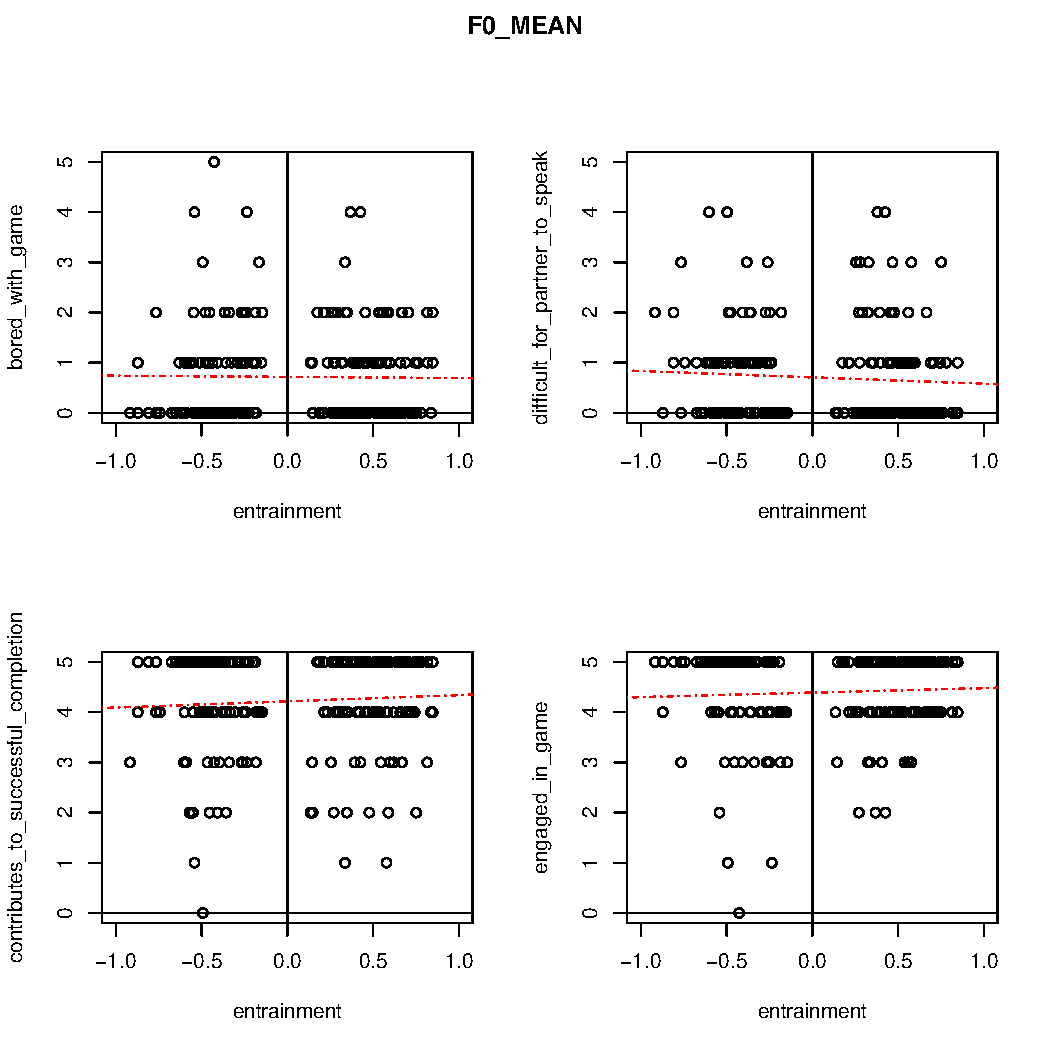
\includegraphics[width=15cm]{images/regression_F0_MEAN_1.pdf}
\caption{Gráfico de los pares entrainment-variable a/p, junto a la regresión lineal obtenida para \emph{F0\_MEAN}}
\label{fig:regresion_clasica}
\end{figure}


% "ENG_MEAN"
% latex table generated in R 3.2.2 by xtable 1.8-0 package
% Thu Jan  7 03:01:56 2016
\begin{tabular}{rrrrr}
  \hline
 ENG\_MEAN & $\widehat{\beta_2}$ & Std. Error & t value & Pr($>$$|$t$|$) \\
  \hline
  bored\_with\_game & 10.6496 & -0 & 2.036037E-21 & 0.6587 \\
  difficult\_for\_partner\_to\_speak & 10.5625 & -1 & 3.728189E-21 & 0.5893 \\
  contributes\_to\_successful\_completion & 59.6193 & -1 & 9.639522E-133 & 0.2519 \\
  engaged\_in\_game & 73.1439 & 1 & 2.276897E-150 & 0.5851 \\
  gives\_encouragement & 47.4920 & -0 & 1.314327E-113 & 0.9659 \\
  making\_self\_clear & 52.9691 & -1 & 1.022216E-122 & 0.3253 \\
  planning\_what\_to\_say & 32.0193 & -2 & 2.465471E-82 & 0.0718 \\
  dislikes\_partner & 9.6126 & -1 & 2.462398E-18 & 0.3482 \\  \hline
\end{tabular}

% latex table generated in R 3.2.2 by xtable 1.8-0 package
% Fri Jan  8 00:50:24 2016
\begin{tabular}{rrrrr}
  \hline
 ENG\_MAX & $\widehat{\beta_2}$ & Std. Error & t value & Pr($>$$|$t$|$) \\
  \hline
bored\_with\_game & 10.4714 & 0 & 7.003232E-21 & 0.9053 \\
  difficult\_for\_partner\_to\_speak & 10.3984 & -0 & 1.160098E-20 & 0.9678 \\
  contributes\_to\_successful\_completion & 58.9660 & -0 & 8.397021E-132 & 0.6739 \\
  engaged\_in\_game & 72.6730 & 1 & 8.299021E-150 & 0.6008 \\
  gives\_encouragement & 47.3103 & -0 & 2.727411E-113 & 0.6494 \\
  making\_self\_clear & 52.2454 & 1 & 1.465061E-121 & 0.3220 \\
  planning\_what\_to\_say & 31.1729 & 0 & 2.491793E-80 & 0.7176 \\
  dislikes\_partner & 9.5924 & -1 & 2.820254E-18 & 0.3279 \\
   \hline
\end{tabular}

% latex table generated in R 3.2.2 by xtable 1.8-0 package
% Thu Jan  7 03:01:56 2016
\begin{tabular}{rrrrr}
  \hline
F0\_MEAN & $\widehat{\beta_2}$ & Std. Error & t value & Pr($>$$|$t$|$) \\
  \hline
bored\_with\_game & 10.6286 & -0 & 2.355933E-21 & 0.8572 \\
  difficult\_for\_partner\_to\_speak & 10.6764 & -1 & 1.689495E-21 & 0.3316 \\
  contributes\_to\_successful\_completion & 59.3792 & 1 & 2.130619E-132 & 0.3726 \\
  engaged\_in\_game & 73.4118 & 1 & 1.094910E-150 & 0.4425 \\
  gives\_encouragement & 47.5948 & 1 & 8.705216E-114 & 0.2774 \\
  making\_self\_clear & 52.9055 & -0 & 1.290163E-122 & 0.7471 \\
  planning\_what\_to\_say & 31.4874 & 0 & 4.441831E-81 & 0.6977 \\
  dislikes\_partner & 9.8092 & -2 & 6.530815E-19 & 0.0835 \\
   \hline
\end{tabular}

% ""
% latex table generated in R 3.2.2 by xtable 1.8-0 package
% Thu Jan  7 03:01:56 2016
\begin{tabular}{rrrrr}
  \hline
F0\_MAX & $\widehat{\beta_2}$ & Std. Error & t value & Pr($>$$|$t$|$) \\
  \hline
bored\_with\_game & 11.0806 & 2 & 1.001502E-22 & 0.0147 \\
  difficult\_for\_partner\_to\_speak & 10.6511 & 1 & 2.014306E-21 & 0.6023 \\
  contributes\_to\_successful\_completion & 60.0792 & -1 & 2.127331E-133 & 0.3297 \\
  engaged\_in\_game & 74.2016 & -1 & 1.282700E-151 & 0.5711 \\
  gives\_encouragement & 48.1664 & -1 & 8.925956E-115 & 0.2986 \\
  making\_self\_clear & 53.8649 & -2 & 3.954497E-124 & 0.0212 \\
  planning\_what\_to\_say & 31.8577 & -1 & 5.915312E-82 & 0.2950 \\
  dislikes\_partner & 9.6545 & 1 & 1.857261E-18 & 0.3340 \\
  \hline
\end{tabular}



\nota{Mover esto a antecedentes}
\section{Valor absoluto de \entrainment}

En nuestra definición de \entrainment en el contexto de series de tiempo, la definimos como el valor de la correlación cruzada (en un sentido de los lags) con mayor valor absoluto. Esto puede dar, como resultado, valores positivos entre 0 y 1 a los cuales consideramos como \entrainment; o bien valores negativos entre -1 y 0, estos considerados como anti-\entrainment: la divergencia de las features a/p medidas a través del tiempo.

Este fenómeno de anti-\entrainment o antimimicry \cite{CHAR1999} refiere al proceso por el cual uno de los interlocutores no imita al otro sino más bien todo lo contrario, acentúa alguna diferencia. Si bien estudios de larga data como \cite{bourhis1973language} o \cite{dabbs1969similarity} lo emparentan con una connotación negativa, \cite{healey2014divergence} y \cite{levitan2015acoustic} sugieren que puede entenderse este fenómeno como una conducta de adaptación cooperativa. No sólo éso, sino que este fenómeno de mimetización complementaria es más prevalente que la mimetización a secas \cite{levitan2015acoustic}.

En base esto es que decidimos probar alguna medida que capture positivamente el fenómeno de la anti-mimetización de igual manera que con el \entrainment antes definido. Es decir, esperamos que cuando tengamos o bien \entrainment o \entrainment complementario ocurra que tenemos valores altos de variables sociales de carácter positivo. Mutatis mutandis con las variables sociales de connotación negativa.

Con este fin, en vez de utilizar sólo el valor de \entrainment como variable explicativa, efectuamos el mismo análisis pero utilizando el valor absoluto del \entrainment como tal. Usar esto permite captar y valorar el \entrainment complementario de la misma manera que el ``positivo'' y valorar su relación con las variables sociales medidas.

\section{Resultados sobre \absentrainment}

\nota{Escribir acá, y poner tablas sobre \absentrainment en pooled}

